\documentclass[english]{mlutalk}
% \documentclass[english,handout]{mlutalk}

\title{Literature Review\\Grimjack at Touché 2021}
\subtitle{Advanced IR, Winter Semester 2021/22}
\author{Johannes Huck \and Jan Heinrich Reimer}
\institute{Martin Luther University Halle-Wittenberg}
\date{\today}
\titlegraphic{
\includegraphics[width=3cm]{figures/mlu-halle}}

\addbibresource{../literature/literature.bib}

\usepackage{tikz}
\usetikzlibrary{positioning}
\usepackage{listings}
\usepackage{xspace}
\usepackage{biblatex}
\usepackage{tabularx}
\usepackage{booktabs}
\usepackage{graphics,graphicx}

\newcommand{\TF}{\mbox{TF}\xspace}
\newcommand{\TFIDF}{\mbox{TF/IDF}\xspace}
\newcommand{\todocite}{{\smaller\color{red}[CITE]}\xspace}
\newcommand{\todo}[1]{{\smaller\color{red}[#1]}}

\lstset{%
  basicstyle=\ttfamily,
  breaklines=true
}

\begin{document}

\titleframe

\begin{frame}{DistilBERT-based Arg. Retrieval~\cite{AlhamzehBEM2021}}
  \begin{itemize}
    \item Touché 2021 participation
    \item Approaches
    \begin{itemize}
      \item Query expansion
      \item Argument extraction
      \item Scoring/sorting
    \end{itemize}
    \item Custom argument identification \\ Not using TARGER~\cite{ChernodubOHBHBP2019}
    \begin{itemize}
      \item Transfer learning
      \item Based on DistilBERT~\cite{SanhDCW2019}
    \end{itemize}
  \end{itemize}
\end{frame}

\begin{frame}[allowframebreaks]{Search pipeline}
  \begin{figure}
    \centering
    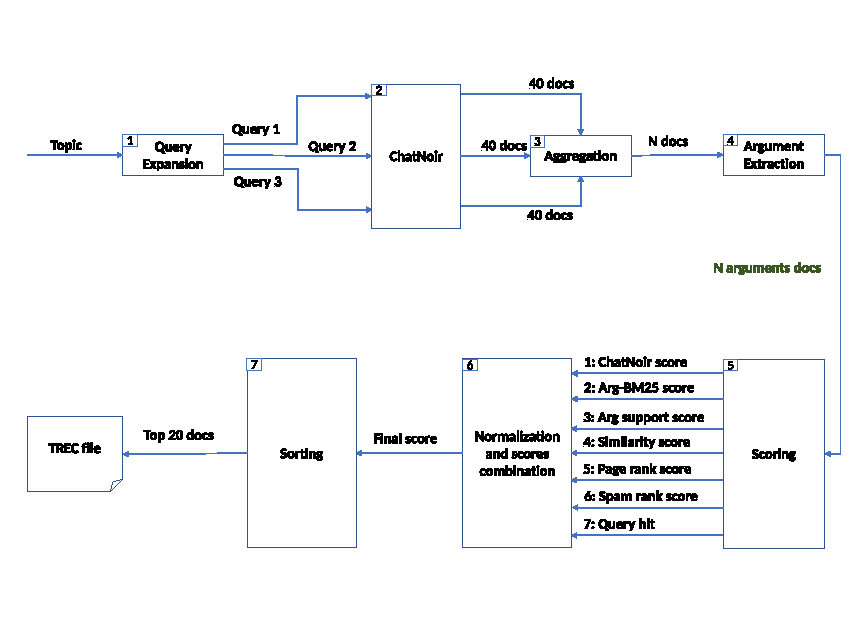
\includegraphics[width=0.8\linewidth]{figures/distilbert-based-arg-retrieval-architecture.pdf}
    \caption{Search pipeline architecture}
    \label{architecture}
  \end{figure}

  \begin{itemize}
    \item TODO
  \end{itemize}
\end{frame}

\begin{frame}{DistilBERT-based Arg. Retrieval~\cite{AlhamzehBEM2021}}
  \begin{figure}
    \centering
    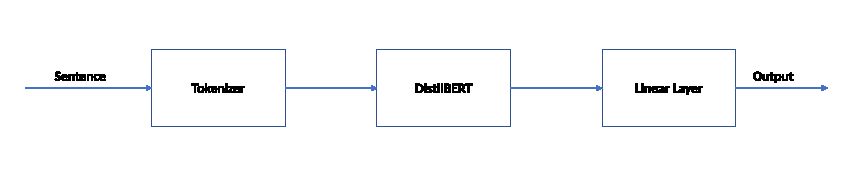
\includegraphics[width=1\linewidth]{figures/distilbert-based-arg-retrieval-processing.pdf}
    \caption{Transfer learning model}
    \label{processing}
  \end{figure}
\end{frame}

\begin{frame}{Conclusion}
  \begin{itemize}
    \item TODO
  \end{itemize}
  \thankyou
\end{frame}

\appendix
\section{\appendixname}

\bibliographyframe

\end{document}